\begin{abstract}
    本文建立了描述信息学比赛的数学模型,并基于该模型研究了过往比赛的选手分数数据。本文通过统计确定了同一名选手的得分波动所服从的分布,基于此从联赛分数推算出了选手整体水平的分布情况,并分析了信息学竞赛选拔流程的效率、回答了有关比赛名次与得分的问题。\emph{上一句待完成后更新。}本文中得到的结论对信息学竞赛赛制的优化、选手的日常训练和比赛策略制定具有参考意义。
\end{abstract}

\section{引言}

    中国高中信息学竞赛的参赛人数和竞赛水平在最近十年中快速提高;这种迅猛的发展在让竞赛趋于繁盛的同时,也使得选手和教练对竞赛现状的认知难以跟上节拍。
    
    这一情况引起了一些问题,例如:

    \begin{asparaitem}
        \item {选手对于自己所处的水平段认识不足,从而作出错误的学业规划。}
        \item {出题人对于选手的水平认识不足,导致题目难度和部分分分配失当。}
        \item {选手不了解对手的水平和发挥情况,导致选择了错误的考场策略。}
    \end{asparaitem}

    本文将利用数学工具,基于过往比赛的选手分数数据来分析信息学竞赛的现状,以为上述问题的解决提供助力。

    \vspace{1.5ex}

    \begin{samepage}
        本文中用到的全部数据可以在以下网址下载:\nobreak
        \begin{compactitem}
            \item {\scriptsize\url{https://files.cnblogs.com/files/turboboost/qty-thesis-statdata.zip}}\nobreak
            \item {\scriptsize\url{https://github.com/TianyiQ/ioi2021-thesis/blob/main/qty-thesis-statdata.zip}}
        \end{compactitem}
    \end{samepage}

    \vspace{1.5ex}

    正文分为五个部分:

    \begin{asparaenum}
        \item [\textbf{第二节}]{建立用于描述信息学比赛的数学模型,作为后续分析的基础。}
        \item [\textbf{第三节}]{分析同一名选手的得分波动所服从的分布。}
        \item [\textbf{第四节}]{利用NOIP初赛、复赛的得分数据推算出信息学竞赛选手整体水平的分布情况。}
        \item [\textbf{第五节}]{\emph{待完成后更新。}}
        \item [\textbf{第六节}]{\emph{待完成后更新。}}
    \end{asparaenum}

    由全文的目标决定,本文将不会对初中信息学竞赛进行研究,因此下文中在提到任何比赛时默认指面向高中生的比赛。

\section{建立模型}

    \subsection{赛程和赛制}

        在引入模型前,先对信息学竞赛的竞赛流程和比赛形式作简要介绍\footnote{赛程和赛制在近几年有小幅变化,本小节中会尽量兼顾新旧两套机制}。

        信息学竞赛是一系列比赛的统称。这些比赛整体上呈现“逐级递进”的关系,即下一层比赛的优胜者晋级上一层比赛。这些比赛按照级别从低到高,大致排列为\footnote{后文将用下表中的字母标号来代指对应的比赛}:

        \begin{asparaenum}[a.]
            \begin{samepage}
            \item 全国联赛(NOIP/CSP)\ ---\ 初赛
            \nobreak
            \item 全国联赛(NOIP/CSP)\ ---\ 复赛
            \nobreak
            \item 省队选拔赛
            \end{samepage}
            \item 清华/北大学科营(THUWC/PKUWC/THUSC/PKUSC)
            \item 亚太地区竞赛(APIO)
            \item 国家队选拔赛(CTSC/CTS)\ ---\ 非正式选手
            \item 全国冬令营(NOIWC)\ ---\ 非正式选手
            \item 全国决赛(NOI)
            \item 清华/北大集训(CTT)
            \begin{samepage}
            \item 全国冬令营(NOIWC)\ ---\ 正式选手
            \nobreak
            \item 国家队选拔赛(CTSC/CTS)\ ---\ 正式选手
            \nobreak
            \item 国际奥林匹克竞赛(IOI)
            \end{samepage}
        \end{asparaenum}

        \begin{figure}
            \centering
            \begin{tikzcd}[column sep=large]
                {} \arrow[r, ">100000"] & a \arrow[d, "20000"]                                     &     \\
                                        & b \arrow[ld, "500"'] \arrow[d, "1000"] \arrow[rd, "500"] &     \\
                d                       & c \arrow[d, "300"] \arrow[l, "300"]                      & efg \\
                                        & h \arrow[d, "70"]                                        &     \\
                                        & ijk \arrow[d, "4"]                                       &     \\
                                        & l                                                        &                 
            \end{tikzcd}
            \caption{信息学比赛间的关系}
            \label{fig:contests}
        \end{figure}

        图\ref{fig:contests}展示了这些比赛间的关系。箭头从低级别比赛指向高级别比赛,表示该低级别比赛的优胜者可以晋级对应的高级别比赛,箭头上标记的数值表示大致晋级人数。

        \vspace{1.5ex}

        赛制即比赛的进行方式和比赛规则。信息学竞赛中采用笔试、COI赛制(机试)、IOI赛制(机试)这三种不同的赛制,表\ref{tab:formats}给出了每种赛制的特点和先前提到的比赛所分别采用的赛制。

        \begin{table}\footnotesize
            \centering
            \begin{tabular}{@{}llllll@{}}
                \toprule
                    & 时长                  & 题数                 & 题目类型       & 反馈机制       & 对应比赛   \\ \midrule
                笔试  & 1\textasciitilde 2h & 数十                 & 选择题、填空题     & 无反馈        & a      \\
                COI赛制 & 3\textasciitilde 5h & 3\textasciitilde 4 & 编程题,有多档部分分 & 无反馈        & bcfghk \\
                IOI赛制 & 3\textasciitilde 5h & 3\textasciitilde 4 & 编程题,有多档部分分 & 多次提交、有反馈 & deijl  \\ \bottomrule
            \end{tabular}
            \caption{信息学比赛采用的赛制}
            \label{tab:formats}
        \end{table}

    \subsection{数学模型}

        本小节中将建立用于描述一场信息学比赛的数学模型。

        \subsubsection{基本模型}
        
            为了更清晰地界定模型在现实中的适用范围,需要先明确:现实中怎样的对象能被称为一场“比赛”。

            \begin{definition}[现实比赛]
                一个\textbf{现实比赛},即特定的人群在同样的规则下测试同一套题目的过程。
                一个现实比赛被\emph{参赛人群}、\emph{规则}和\emph{题目}这三个要素所确定。
                \label{def:realContest}
            \end{definition}

            在这一定义下,每年中的 $a\sim l$ 这12个比赛,自然都是现实比赛。而且,不仅是包含两天考试的一场完整的比赛算作现实比赛,单独拿出其中一天也算现实比赛。
            
            \vspace{1.5ex}

            关于“参赛人群”这一概念需要注意两点:
            
            \begin{asparaitem}
                \item 参赛人群只是一个宽泛的范围,而不是具体的选手集合。例如我们可以规定参赛人群为“所有学习信息学的同学”,但这一规定并不关注张三、李四、王五是否是这个人群的成员。这样的规定不会给后续的分析带来不利影响,因为我们只关心关于比赛和人群的统计信息,而不关心每名选手的特点。
                \item 参赛人群不必囊括实际参赛的整个选手群体;例如在NOIP初赛中,“所有报名了初赛的女生”这一参赛群体依然能构成现实比赛。这一点对于后文中跨越不同比赛的分析大有帮助。
            \end{asparaitem}
            
            \vspace{1.5ex}

            接下来定义从现实比赛抽象而来的数学模型。

            \begin{definition}[理想比赛]
                \textbf{理想比赛} $A$ 由二元函数 $\bm{H}_A:\left[0,1\right]\times\mathbb{R}\to\mathbb{R}_{\geq 0}$ 确定,其中 $\bm{H}_A$ 连续且满足
                \begin{equation}
                    \int\limits_0^1\int\limits_{-\infty}^{+\infty} \bm{H}_A(x,\delta)\mathrm{d}\delta\mathrm{d}x=1
                    \label{formula:totalEqual1}
                \end{equation}
                和
                \begin{equation}
                    \int\limits_{-\infty}^{+\infty} \delta\cdot\bm{H}_A(x_0,\delta)\mathrm{d}\delta=0,\quad\forall x_0\in\left[0,1\right]
                    \label{formula:expectationEqual0}
                \end{equation}
                此时我们把 $\bm{H}_A$ 称为 $A$ 的\textbf{综合分布函数}。
                \label{def:idealContest}
            \end{definition}

            接下来将定义:一个理想比赛何时被认为“描述”了一个现实比赛。这也将同时表明综合分布函数的实际含义。
            
            \vspace{1.5ex}

            首先约定一下记号:

            \begin{asparaitem}
                \item $\mathrm{Pr}\left[A\right]$ 表示事件 $A$ 发生的概率。
                \item $\mathrm{E}\left[X\right]$ 表示随机变量 $X$ 的期望值。
            \end{asparaitem}

            \begin{definition}
                从现实比赛 $B$ 可按如下方式确定一个理想比赛 $A$ :

                \begin{asparaenum}[\bfseries{步骤} 1.]
                    \item 记 $B$ 的参赛选手集合为有限集 $S_B$ ,并在 $B$ 的参赛人群(包括人群内部的具体构成)不变的情况下,假想参赛人数 $\left|S_B\right|$ 趋于无穷。我们之所以能够任意钦定 $\left|S_B\right|$ ,是因为——如先前所述——$B$的定义并未指明具体的选手集合。
                    \item \label{step:realToIdealStep2} 每一名参赛选手 $p$ 在比赛 $B$ 中的实际得分 $\textit{score}_p$ 是一个随机变量,它被各种偶然因素(如临场发挥)所支配,但是它的分布可以由选手 $p$ 和现实比赛 $B$ 的三个要素完全确定。假想对每一名选手 $p$ 计算其期望得分 $\textit{exscore}_p=\mathrm{E}\left[\textit{score}_p\right]$ ,并取所有选手期望得分的最大值,记作 $M_B$ 。由于参赛人数趋于无穷,每一个个人的特征可以忽略,故 $M_B=\max\limits_{p\in S_B} \textit{exscore}_p$ 仅由 $B$ 确定。
                    \item \label{step:realToIdealStep3} 从 $S_B$ 中等概率随机选取一名选手 $p$ ,并:
                    \begin{itemize}[leftmargin=4em]
                        \item 定义 $[0,1]$ 上的随机变量 $X_B=\frac{\textit{exscore}_p}{M_B}$ 。\footnote{“将每名选手的分数除以最高分数”这一操作,类似于信息学比赛中计算标准分的方式。另外注意到:虽然 $\frac{\textit{exscore}_p}{M_B}\leq 1$ ,但 $\frac{\textit{score}_p}{M_B}$ 可以大于 $1$ }易见随机变量 $X_B$ 的实际取值与考场上的偶然因素无关,而是由选取 $p$ 的方式确定。
                        \item 定义 $\mathbb{R}$ 上的随机变量 $\Delta_B=\frac{\textit{score}_p-\textit{exscore}_p}{M_B}$ 。易见随机变量 $\Delta_B$ 的实际取值由选取 $p$ 的方式和考场上的偶然因素(如选手临场发挥)共同确定。
                        \item [◦] 请注意,$X_B$ 和 $\Delta_B$ 的定义中所用的 $p$ 是\emph{同一名}随机选择的选手,而不是独立的两次选择。
                    \end{itemize}
                    \item 取 $A$ 的综合分布函数 $\bm{H}_A$ 为 $X_B$ 与 $\Delta_B$ 的联合概率密度函数,从而确定 $A$ 。换句话说,对所有 $x_0\in[0,1],\delta_0\in\mathbb{R}$ ,需要满足\footnote{也可以直观地理解为$\bm{H}_A(x_0,\delta_0)=\mathrm{Pr}\left[\left(X_B\approx x_0\right)\land\left(\Delta_B\approx\delta_0\right)\right]$,不写作 $X_B=x_0$ 是因为取等概率为 $0$ }
                    \begin{equation}
                        \int\limits_0^{x_0}\int\limits_{-\infty}^{\delta_0} \bm{H}_A(x,\delta)\mathrm{d}\delta\mathrm{d}x=\mathrm{Pr}\left[\left(X_B\leq x_0\right)\land\left(\Delta_B\leq\delta_0\right)\right]
                        \label{formula:definitionOfJointDensityFunction}
                    \end{equation}

                \end{asparaenum}

                由\eqref{formula:definitionOfJointDensityFunction}知定义\ref{def:idealContest}的等式\eqref{formula:totalEqual1}满足;由 $\mathrm{E}\left[\Delta_B\right]=0$ 知等式\eqref{formula:expectationEqual0}满足。从而只要联合概率密度函数 $\bm{H}_A$ 存在且连续, $A$ 就符合理想比赛的定义。

                对于按上述方式得到的 $A$ ,我们称 $A$ 与 $B$ \textbf{互相对应}。如果按上述过程得到的 $\bm{H}_A$ 不连续或根本不存在,则认为不存在与 $B$ 对应的 $A$ 。
                
                \label{def:realIdealCorrespondence}
            \end{definition}

            冗长的定义可以用一句话来作直观的总结:$\bm{H}_A\left(x,\delta\right)$ 表示真实水平(即期望得分)约为 $x$ ($x\in\left[0,1\right]$为按最高分折算后的标准分)、实际表现约为 $x+\delta$ (同样表示标准分)的选手的\emph{期望}人数占总人数的比例;之所以实际表现会偏离真实水平——以及这里之所以说“期望人数”——是因为考场上的各种偶然因素为比赛结果带来了随机性。

            可以看到,理想比赛这一模型只考虑了哪些结果\emph{可能}出现,而未考虑哪种结果\emph{实际}出现。而在现实中,能够获知的却只有实际出现的结果——和它恰恰相反。下面定义的概念将处理这一问题。

            \begin{definition}[分数分布函数]
                对理想比赛 $A$ ,定义其\textbf{分数分布函数} $\bm{C}_A:\mathbb{R}\to\mathbb{R}_{\geq 0}$ 满足
                $$
                \bm{C}_A(s)=\int\limits_{0}^1 \bm{H}_A(x,s-x) \mathrm{d}x,\quad\forall s\in\mathbb{R}
                $$

                \label{def:scoreDistribution}
            \end{definition}

            \begin{proposition}[分数分布函数的实际含义]
                对现实比赛 $B$ 和与之对应的理想比赛 $A$ ,假想比赛 $B$ 的参赛人数 $|S_B|$ 趋于无穷,等概率随机选取选手 $p\in S_B$ ,则\footnote{也就是说 $\bm{C}_A$ 为随机变量 $\frac{\textit{score}_p}{M_B}$ 的概率密度函数。和先前类似,这里也可以直观理解为 $\bm{C}_A(r)=\mathrm{Pr}\left[\frac{\textit{score}_p}{M_B}\approx r\right]$ }:
                $$
                \mathrm{Pr}\left[\frac{\textit{score}_p}{M_B}\leq r\right]=\int\limits_{-\infty}^r \bm{C}_A(s)\mathrm{d}s,\quad\forall r\in\mathbb{R}
                $$

                \label{prop:scoreDistributionMeaning}
            \end{proposition}

            \begin{proof}
                \begin{align*}
                    \mathrm{Pr}\left[\frac{\textit{score}_p}{M_B}\leq r\right]
                    &=\mathrm{Pr}\left[X_B+\Delta_B\leq r\right] \\
                    &=\iint\limits_{\left\{(x,\delta):x\in\left[0,1\right],\delta\in\mathbb{R},x+\delta\leq r\right\}}\bm{H}_A(x,\delta)\mathrm{d}(x,\delta) \\
                    &=\iint\limits_{\left\{(x,s):x\in\left[0,1\right],s\in\left(-\infty,r\right]\right\}}\bm{H}_A(x,s-x)\mathrm{d}(x,s) \\
                    &=\int\limits_{-\infty}^r\left(\int\limits_0^1 \bm{H}_A(x,s-x)\mathrm{d}x\right)\mathrm{d}s \\
                    &=\int\limits_{-\infty}^r \bm{C}_A(s)\mathrm{d}s
                \end{align*}
            \end{proof}

            在上面四个定义中,涉及到现实情况的部分难免有模糊之处;实际应用中对这几条定义的执行,也不可避免地需要作近似处理。但即便如此,作出这些规定依然能极大地帮助我们厘清思路并发现隐含的前提。

        \subsubsection{特殊情况下的模型}

            在一场现实比赛 $B$ 中,每一个选手 $p\in S_B$ 的实际得分相比真实水平的“得分偏移量” $\frac{\textit{score}_p-\textit{exscore}_p}{M_B}$ 都是一个随机变量。如果所有选手的“得分偏移量”独立同分布,对我们的模型意味着什么?

            容易想到,此时随机变量 $\Delta_B$ 的概率分布就和任何一个选手的“得分偏移量”的概率分布完全相同。换句话说,在定义\ref{def:realIdealCorrespondence}的步骤\ref{step:realToIdealStep3}中,不论我们钦定选取哪一个 $p$ , $\Delta_B$ 取任何一个值的概率都是固定的,且恰好等于在不固定 $p$ 的情况下 $\Delta_B$ 取这个值的概率。再换句话说\footnote{和之前类似,这里之所以不写 $\Delta_B=\delta$ ,是因为取等概率为 $0$ }:$$\mathrm{Pr}\left[(\Delta_B\leq\delta)|(X_B=x)\right]=\mathrm{Pr}\left[\Delta_B\leq\delta\right],\ \forall \left(\delta\in\mathbb{R},x\in\left[0,1\right],\mathrm{Pr}\left[X_B=x\right]>0\right)$$即随机变量 $X_B,\Delta_B$ 独立。在研究这件事之前,我们需要一对新的定义。

            \begin{definition}[期望值分布函数和偏移量分布函数]
                对任意的理想比赛 $A$ :
                \begin{asparaitem}
                    \item 定义其\textbf{期望值分布函数} $\bm{X}_A:[0,1]\to\mathbb{R}_{\geq 0}$ 满足 $$\bm{X}_A(x_0)=\int\limits_{-\infty}^{+\infty}\bm{H}_A(x_0,\delta)\mathrm{d}\delta,\quad\forall x_0\in[0,1]$$
                    \item 定义其\textbf{偏移量分布函数} $\bm{\Delta}_A:\mathbb{R}\to\mathbb{R}_{\geq 0}$ 满足 $$\bm{\Delta}_A(\delta_0)=\int\limits_0^1\bm{H}_A(x,\delta_0)\mathrm{d}x,\quad\forall\delta_0\in\mathbb{R}$$
                \end{asparaitem}
                \label{def:marginalDistributions}
            \end{definition}

            \begin{proposition}[期望值分布函数和偏移量分布函数的实际含义]
                对现实比赛 $B$ 和与之对应的理想比赛 $A$ :
                \begin{asparaitem}
                    \item $\bm{X}_A$ 为 $X_B$ 的概率密度函数。换句话说\footnote{也可以直观地理解为:$\mathrm{Pr}[X_B\approx x_0]=\bm{X}_A(x_0)$}:$$\mathrm{Pr}[X_B\leq x_0]=\int\limits_0^{x_0} \bm{X}_A(x)\mathrm{d}x,\quad\forall x_0\in[0,1]$$
                    \item $\bm{\Delta}_A$ 为 $\Delta_B$ 的概率密度函数。换句话说\footnote{也可以直观地理解为:$\mathrm{Pr}[\Delta_B\approx \delta_0]=\bm{\Delta}_A(\delta_0)$}:$$\mathrm{Pr}[\Delta_B\leq \delta_0]=\int\limits_{-\infty}^{\delta_0} \bm{\Delta}_A(\delta)\mathrm{d}\delta,\quad\forall \delta_0\in\mathbb{R}$$
                \end{asparaitem}
                \label{prop:marginalDistributionsMeaning}
            \end{proposition}

            证明比较显然,这里略去。下面考虑 $X_B,\Delta_B$ 间的独立性带来的性质。

            \begin{proposition}
                对现实比赛 $B$ 和与之对应的理想比赛 $A$ ,如果 $X_B$ 与 $\Delta_B$ 独立,则:
                \begin{equation}
                    \bm{H}_A(x_0,\delta_0)=\bm{X}_A(x_0)\bm{\Delta}_A(\delta_0),\quad\forall (x_0,\delta_0)\in[0,1]\times\mathbb{R}
                    \label{formula:insideImplicationOfIndependence}
                \end{equation}

                更进一步,\eqref{formula:insideImplicationOfIndependence}是 $X_B$ 与$\Delta_B$ 独立的充要条件。

                \label{prop:implicationOfIndependence}
            \end{proposition}

            \begin{proof}
                \begin{align*}
                    &\phantom{\Leftrightarrow\ }\mathrm{Pr}\left[(\Delta_B\leq\delta_0)|(X_B=x_0)\right]=\mathrm{Pr}\left[\Delta_B\leq\delta_0\right],\ \forall \left(\delta_0\in\mathbb{R},\mathrm{Pr}\left[X_B=x_0\right]>0\right) \\
                    &\Leftrightarrow \left(\displaystyle\int\limits_{-\infty}^{\delta_0} \bm{H}_A(x_0,\delta)\mathrm{d}\delta\right)\Big/{\bm{X}_A(x_0)}=\int\limits_{-\infty}^{\delta_0} \bm{\Delta}_A(\delta)\mathrm{d}\delta,\ \forall \left(\delta_0\in\mathbb{R},\bm{X}_A(x_0)>0\right)\\
                    &\Leftrightarrow \frac{\bm{H}_A(x_0,\delta_0)}{\bm{X}_A(x_0)}=\bm{\Delta}_A(\delta_0),\ \forall \left(\delta_0\in\mathbb{R},\bm{X}_A(x_0)>0\right)\\
                    &\Leftrightarrow \eqref{formula:insideImplicationOfIndependence}
                \end{align*}
                
                最后一步中还需要特别考虑 $\bm{X}_A(x_0)=0$ 的情况,不难自行补全。
            \end{proof}

            \begin{definition}[简单理想比赛]
                如果理想比赛 $A$ 满足 \eqref{formula:insideImplicationOfIndependence} 式,则称它是\textbf{简单}的。

                \label{def:simplicityOfContest}
            \end{definition}

            由命题\ref{prop:implicationOfIndependence},对于简单理想比赛 $A$ ,从 $\bm{X}_A,\bm{\Delta}_A$ 可唯一确定 $\bm{H}_A$ ,进而能够确定 $\bm{C}_A$ 。

            \begin{proposition}[简单理想比赛的分数分布函数]
                对简单理想比赛 $A$ :
                $$
                \bm{C}_A(s)=\int\limits_{0}^1 \bm{X}_A(x)\bm{\Delta}_A(s-x) \mathrm{d}x,\quad\forall s\in\mathbb{R}
                $$

                \label{def:scoreDistributionInSimpleContest}
            \end{proposition}

            证明显然,这里略去。

    \subsection{几个关键的假设}

        为了使得后续分析成为可能,我们还需要对真实情况作一些近似处理。近似处理的具体方式由本小节的几个假设给出。

        \begin{assumption}
            对任何一个信息学(现实)比赛 $B$ ,都存在符合定义\ref{def:idealContest}的理想比赛 $A$ 与其对应。

            \label{ass:existenceOfIdealContest}
        \end{assumption}

        \begin{assumption}
            对任何一个现实比赛,如果它的\emph{规则}基于COI或IOI赛制,则它对应的理想比赛是简单的。

            \label{ass:simplicityOfCodingContests}
        \end{assumption}

        \begin{assumption}
            考虑所有基于COI或IOI赛制的现实比赛,考察它们对应的理想比赛的偏移量分布,这些分布应该是\emph{相似}的,即它们应该有相同的形式,即使其中的参数可能有不同的取值。

            \label{ass:similarityOfDeltaDistributions}
        \end{assumption}

        在给出下一个假设之前,还需要定义一个概念。

        \begin{definition}[缩放等价]
            对简单理想比赛 $A_1,A_2$ ,当存在线性映射 $f(x)=\alpha x+\beta\quad(\alpha\in\mathbb{R}_{> 0},\beta\in\mathbb{R})$ 同时满足以下条件时,称 $A_1,A_2$ \textbf{缩放等价},称 $f$ 为 $A_1,A_2$ 间的\textbf{等价映射}:
            \begin{asparaenum}
                \item $f(1)=1$
                \item $\bm{\Delta}_{A_2}(\alpha\delta)=\bm{\Delta}_{A_1}(\delta)\cdot \alpha^{-1},\quad\forall \delta\in\mathbb{R}$
                \item $\widebar{\bm{X}}_{A_2}(f(x))=\widebar{\bm{X}}_{A_1}(x)\cdot \alpha^{-1},\quad\forall x\in\mathbb{R}$ ,其中
                    $$
                        \widebar{\bm{X}}(x)=
                        \begin{cases} 
                            0 & x\notin [0,1] \\
                            \bm{X}(x) & x\in[0,1]
                        \end{cases}
                    $$
            \end{asparaenum}

            \label{def:equivalenceAfterScaling}
        \end{definition}

        \begin{proposition}[缩放等价的实际含义]
            对缩放等价的 $A_1,A_2$ 及其等价映射 $f$ ,有以下关系\footnote{可以直观理解为:现实比赛 $B_1$ (对应于 $A_1$ )中的分数,经过 $f:x\mapsto\alpha x+\beta$ 的变换之后,变成了现实比赛 $B_2$ (对应于 $A_2$ )中的分数}:
            \begin{asparaenum}
                \item $\displaystyle\int\limits_{-\infty}^{\delta_0} \bm{\Delta}_{A_1}(\delta)\mathrm{d}\delta=\displaystyle\int\limits_{-\infty}^{\alpha\delta_0} \bm{\Delta}_{A_2}(\delta)\mathrm{d}\delta,\quad\forall\delta\in\mathbb{R}$
                \item $\displaystyle\int\limits_{-\infty}^{x_0} \widebar{\bm{X}}_{A_1}(x)\mathrm{d}x=\displaystyle\int\limits_{-\infty}^{f(x_0)} \widebar{\bm{X}}_{A_2}(x)\mathrm{d}x,\quad\forall x\in\mathbb{R}$
            \end{asparaenum}

            \label{prop:equivalenceAfterScalingMeaning}
        \end{proposition}

        \begin{proof}
            先来看关于 $\bm{\Delta}_{A_1},\bm{\Delta}_{A_2}$ 的部分:
            \begin{align*}
                \int\limits_{-\infty}^{\delta_0} \bm{\Delta}_{A_1}(\delta)\mathrm{d}\delta 
                &=\int\limits_{-\infty}^{\delta_0} \bm{\Delta}_{A_2}(\alpha\delta)\alpha\mathrm{d}\delta \\
                &=\int\limits_{-\infty}^{\alpha\delta_0} \bm{\Delta}_{A_2}(\alpha\delta)\alpha \mathrm{d}(\alpha\delta)\cdot\alpha^{-1} \\
                &=\int\limits_{-\infty}^{\alpha\delta_0}\bm{\Delta}_{A_2}(t)\mathrm{d}t
            \end{align*}

            对于 $\widebar{\bm{X}}_{A_1},\widebar{\bm{X}}_{A_2}$ 同理,这里不再重复。
        \end{proof}

        \begin{assumption}
            对现实比赛 $B_1$ (对应理想比赛 $A_1$ )和 $B_2$ (对应理想比赛 $A_2$ ),如果 $B_1,B_2$ 的\emph{规则}都基于COI或IOI赛制,且它们的\emph{参赛人群}相同,则 $A_1,A_2$ 一定缩放等价。
            \label{ass:equivalenceBetweenCodingContests}
        \end{assumption}

        对这些假设无法予以严格的证明,但在此可以列举一些感性的理由,来说明它们大体上是可靠的。

        \begin{asparaenum}
            \item \label{step:argumentForAssumptionStep1} 如果假设所有比赛在考查角度上没有差异(因为我们只关心普遍的统计特征,所以这种假设是合理的),那么一名选手的解题能力(即,能够在比赛中解出多大难度的题目)就一定是固定的。
            \item \label{step:argumentForAssumptionStep2} 当组题人为一场比赛选择题目、出题人为命制的题目设置部分分时,他们会有意识地给较难的任务设置较高的分值、给较简单的任务设置较低的分值,而具体多高、多低,则取决于他们心中作的判断。虽然不同的人可能作出不一样的判断,但这些判断应该大体上是“成比例”的。例如:张三认为算法2应当获得三倍于算法1的得分、李四认为算法2应当获得2.5倍于算法1的得分,这两种判断在比例上是大致相符的。
            \item 综合\ref{step:argumentForAssumptionStep1}和\ref{step:argumentForAssumptionStep2},我们知道了:每个选手的能力可以看作是不变的;选手比赛中完成的任务难度与所获分数间的关系,这一关系在不同比赛之间应该是“成比例”的。所以只要选手集合不变,不同比赛的“选手期望得分构成的分布”也应该是“成比例”的(特别地,这两个分布的最大值也应该是相对应的,所以在定义\ref{def:equivalenceAfterScaling}中要求$f(1)=1$)。这就为假设\ref{ass:equivalenceBetweenCodingContests}关于期望值分布的部分和对 $f(1)=1$ 的要求提供了依据。
            \item 根据经验,一名选手考场发挥的稳定与否与水平高低等因素没有明显的相关性;所以虽然不同选手的稳定性存在差异,但是在样本很大时,这种差异不会给统计结果带来较大的系统性的偏差,因此我们近似地认为所有选手\emph{水平发挥}的稳定性是相同的。又因为得分与实际表现出的能力是“成比例”的,所以所有选手\emph{比赛得分}的稳定性也是相同的。这为假设\ref{ass:simplicityOfCodingContests}、假设\ref{ass:similarityOfDeltaDistributions}和假设\ref{ass:equivalenceBetweenCodingContests}关于偏移量分布的部分提供了依据。
            \item 真实的比赛中“离散”的特性——比如选择题三分一道——可以在理想化的模型中忽略。这样在人数趋于无穷时,我们很容易想到:其各种统计数据会是“连续”的。因此\ref{ass:existenceOfIdealContest}是一个很自然的假设。
            \item 根据经验,在COI赛制中表现好的选手,在IOI赛制往往表现也很好;反之亦然。因此COI/IOI赛制间的差异至多会对选手期望得分的分布起到缩放的作用,而不会带来本质的改变。类似地,选手在COI/IOI赛制中发挥稳定性的差异,也只有量的差别而无质的差别。所以,认为COI/IOI赛制的比赛有着本质相同(即在缩放后完全相同)的期望值分布、偏移量分布,是合理的。
        \end{asparaenum}

\section{偏移量分布的测量}

    由假设\ref{ass:similarityOfDeltaDistributions},COI/IOI赛制下偏移量分布有一定的形式。本节中,将利用过往比赛的分数数据得到偏移量分布的形式。

    \subsection{数据的获取}

        数据来自以下三场比赛:
        \begin{asparaitem}
            \item 2018年北大集训(字母标号i)
            \item 2019年北大集训(字母标号i)
            \item 2020年北大集训(字母标号i)
        \end{asparaitem}

        选用它们的原因是,北大集训包含连续进行的四场考试,更多的考试场数使得我们能够更精确地估计每一名选手的期望分数。

        这些比赛的参赛情况见表\ref{tab:ctt18to20}。

        \begin{table}\footnotesize
            \centering
            \begin{tabular}{@{}lcccc@{}}
            \toprule
             & \multicolumn{1}{l}{参赛总人数} & \multicolumn{1}{l}{正式选手人数} & \multicolumn{1}{l}{非正式选手人数} & \multicolumn{1}{l}{选拔人数} \\ \midrule
            北大集训2018 & 约60 & 50 & 约10 & 15 \\
            北大集训2019 & 约70 & 50 & 约20 & 15 \\
            北大集训2020 & 约90 & 50 & 约40 & 30 \\ \bottomrule
            \end{tabular}
            \caption{三场比赛的参赛情况}
            \label{tab:ctt18to20}
        \end{table}

        根据经验判断,这三场比赛中并非所有选手都全情投入。因此为了保证数据可靠性,对每场比赛只取总排名\footnote{总排名中按每天标准分总和降序排列}中最靠前的 $1.5K\sim 2K$ 名选手的数据,其中 $K$ 表示当场比赛的选拔人数。具体地说:北大集训2018取前30名、北大集训2019取前30名、北大集训2020取前50名。另外为保证比赛之间的统一性,后文中在计算考试分数标准差时,每场比赛只取总排名中前30名的分数。

    \subsection{数据的加工处理}\label{sec:dataPreprocessingOfCTT}

        三场比赛的参赛选手共计110人次,我们将他们视为110名不同的选手。三场比赛共计12场考试,我们将它们视为12个不同的现实比赛。参加这些现实比赛的共计440人次。
        
        虽然这12个现实比赛的参赛人群是相同的(国家集训队选手和精英培训选手),但它们在题目难度等方面并不相同,如果直接将它们的数据汇总起来的话,会使得数据失去意义。为解决这一问题,我们需对比赛得分进行变换。

        \begin{proposition}
            对缩放等价的理想比赛 $A_1,A_2$ 及其等价映射 $f(x)=\alpha x+\beta$\nobreak,有
            $$
            \alpha=\frac{\mathrm{Stddev}\left[\bm{C}_{A_2}\right]}{\mathrm{Stddev}\left[\bm{C}_{A_1}\right]}
            $$
            其中 $\mathrm{Stddev}\left[F\right]$ 表示以 $F$ 为概率密度函数的随机变量\footnote{换句话说,这样的随机变量 $Y$ 满足 $\mathrm{Pr}\left[Y\leq t\right]=\int\limits_{-\infty}^t F(s)\mathrm{d}s,\quad\forall t\in\mathbb{R}$}的标准差。

            另外注意到由 $f(1)=1$ 可得 $f(x)=1-\alpha(1-x)$ ,所以不必再考虑 $\beta$ 的取值。
            \label{prop:alphaAsQuotientOfStddev}
        \end{proposition}

        \begin{proof}
            \begin{align*}
                \bm{C}_{A_1}(s)
                &=\int\limits_0^1 \bm{X}_{A_1}(x)\bm{\Delta}_{A_1}(s-x) \mathrm{d}x \\
                &=\int\limits_{-\infty}^{+\infty} \bm{X}_{A_1}(x)\bm{\Delta}_{A_1}(s-x) \mathrm{d}x \\
                &=\int\limits_{-\infty}^{+\infty} \left(\widebar{\bm{X}}_{A_2}(\alpha x+\beta)\cdot\alpha\right)\left(\bm{\Delta}_{A_2}(\alpha(s-x))\cdot\alpha\right) \mathrm{d}x\\
                &=\int\limits_{-\infty}^{+\infty} \alpha^2\widebar{\bm{X}}_{A_2}\left(\alpha x+\beta\right)\bm{\Delta}_{A_2}\left(\alpha s+\beta-\left(\alpha x+\beta\right)\right) \mathrm{d}(\alpha x+\beta)\cdot\alpha^{-1}\\
                &=\alpha\int\limits_{-\infty}^{+\infty} \widebar{\bm{X}}_{A_2}(t)\bm{\Delta}_{A_2}((\alpha s+\beta)-t)\mathrm{d} t\\
                &=\alpha\bm{C}_{A_2}(\alpha s+\beta),\quad\forall s\in\mathbb{R}
            \end{align*}

            设连续型随机变量 $Y_1$ 满足其概率密度函数为 $\bm{C}_{A_1}$ ,$Y_2$ 满足其概率密度函数为 $\bm{C}_{A_1}$ ,则 $\alpha Y_1+\beta$ 与 $Y_2$ 同分布。从而\footnote{这里 $\mathrm{Var}\left[Y\right]$ 表示随机变量 $Y$ 的方差} $\mathrm{Var}\left[Y_2\right]=\mathrm{Var}\left[\alpha Y_1\right]=\alpha^2\cdot\mathrm{Var}\left[Y_1\right]$ ,于是 $\mathrm{Stddev}\left[Y_2\right]=\alpha\cdot\mathrm{Stddev}\left[Y_1\right]$ 。
        \end{proof}

        结合等价映射的实际含义和命题\ref{prop:alphaAsQuotientOfStddev},可以得到对前述12个现实比赛 $B_{1\cdots 12}$ 的分数做变换的方法:
        \begin{asparaenum}[\bfseries{步骤} 1.]
            \item 记 $B_{1\cdots 12}$ 对应的理想比赛为 $A_{1\cdots 12}$ 。
            \item 构造 $A^{\prime}_{1\cdots 12}$ 满足 $A_i$ 与 $A^{\prime}_i$ 缩放等价,且等价映射为 $f_i(x)=1-\frac{1-x}{c\cdot\mathrm{Stddev}\left[\bm{C}_{A_i}\right]}$ 。这里 $c=4$ 为根据实际数据所选取的固定常数,用来避免产生负分数。
            \item 则 $A^{\prime}_{1\cdots 12}$ 这12个理想比赛完全相同(即它们的综合分布函数相同),且与 $A_{1\cdots 12}$ 中的每一个缩放等价。
        \end{asparaenum}

        \vspace{1.5ex}

        另外须注意,根据定义\ref{def:realIdealCorrespondence}的步骤\ref{step:realToIdealStep2},我们需要对每个现实比赛 $B_i$ 确定选手期望分数的最大值 $M_{B_i}$ 。这里可以用实际分数的最大值来近似地代替期望分数的最大值。
        
        因为 $A^{\prime}_{1\cdots 12}$ 与 $A_{1\cdots 12}$ 中的每一个缩放等价,所以我们只需测量 $A^{\prime}_{1\cdots 12}$ 的偏移量分布,即可得到结论。现在开始目标将转为测量 $A^{\prime}_{1\cdots 12}$ 的偏移量分布;为便于表述,记 $B^{\prime}_{1\cdots 12}$ 表示 $A^{\prime}_{1\cdots 12}$ 对应的现实比赛。

        现在我们得到了12个完全相同的理想比赛 $A^{\prime}_{1\cdots 12}$ ,和每个理想比赛对应的现实比赛的分数数据;而因为 $A^{\prime}_{1\cdots 12}$ 完全相同,所以所有这些分数数据可以直接合并。现在我们有了一个理想比赛(记为$A^{\prime}$,对应现实比赛 $B^{\prime}$)和对应的440名选手的分数数据。原先的110名选手,每人对应着 $B^{\prime}$ 中的4名选手。

        对于110名选手中的每一位,为了能够对比他在 $B^{\prime}$ 中的期望分数和他的四个“分身”的实际分数,我们还需要估算前者的值。这里可以用该名选手在他所参加的4场现实比赛 $B^{\prime}_i$ 中的平均分,来近似地代替在 $B^{\prime}$ 中的期望分数。

        \vspace{1.5ex}

        综上所述,我们会按如下的流程来加工分数数据:
        \begin{asparaenum}[\bfseries{步骤} 1.]
            \item \label{step:cttDataRefinementStep1} 对12场考试中的每一场,将其中每一名选手的分数除以该场考试的最高分\footnote{即信息学比赛中计算标准分的过程},并以此代替原始分数。
            \item 对12场考试中的每一场,计算总排名前30的选手的分数标准差 $\sigma$ (这里的分数是指步骤\ref{step:cttDataRefinementStep1}中得到的商),然后将其中每个选手的分数 $x$ 施以变换\footnote{除以标准差这一步的作用也可简单理解为,消除题目区分度不同所带来的影响} $x\mapsto 1-\frac{1-x}{4\sigma}$ ,并以此代替原始分数。
            \item 对110名选手中的每一位,计算他在4场考试中的平均分,然后计算他在每场考试中的得分与这一平均分的差。
        \end{asparaenum}

        \vspace{1.5ex}

        这样可以对每名选手计算出4个差值,共计440个值,每个值都表示一名选手在一场比赛中实际得分与期望得分的差距。这440个值即对应着随机变量 $\Delta_{B^{\prime}}$ 的取值,它们将会是下一小节的分析对象。

    \subsection{拟合的方法和结果}

        观察上一小节中获得的440个数值的分布情况,发现:
        \begin{asparaitem}
            \item 整个分布大体上对称,且以$0$为对称中心。
            \item 数值的分布中间稠密、两边稀疏,所有数值的绝对值都小于1。
            \item 分布的形状类似钟形曲线。
        \end{asparaitem}
        
        \vspace{1.5ex}

        受此启发,尝试用正态分布曲线来拟合这些数值。具体方法如下:
        \begin{enumerate}[leftmargin=6em]
            \item [\textbf{步骤 1.}] 对于 $t=-1.0,-0.9,\cdots,1.0$ ,计算:落在 $\left[t-0.05,t+0.05\right)$ 中的数值个数与总个数440的比值。这个比值记作 $c(t)$ 。
            \item [\textbf{步骤 2.}] 在平面直角坐标系中画出 $t-c(t)$ 散点图。
            \item [\textbf{步骤 3.}] 选取合适的参数 $\sigma>0$ ,以使得函数 $$ f(t)=\displaystyle\int\limits_{t-0.05}^{t+0.05} P_{\sigma^2}(x)\mathrm{d} x$$ 的图像与这些 $t-c(t)$ 数据点尽可能贴近。
        \end{enumerate}

        这里 $P_{\sigma^2}$ 表示期望值为0、方差为 $\sigma^2$ 的正态分布(用 $N(0,\sigma^2)$ 表示)的概率密度函数,满足 $$P_{\sigma^2}(x)=\frac{1}{\sqrt{2\pi}\sigma}\exp{\left(-\frac{x^2}{2\sigma^2}\right)}$$

        再记 $$R_{\sigma^2}(t)=\int\limits_{-\infty}^t P_{\sigma^2}(x)\mathrm{d}x$$ 为正态分布 $N(0,\sigma^2)$ 的累积分布函数,则有\footnote{误差函数 $\mathrm{erf}$ 没有闭合形式,这个式子可以视为$\mathrm{erf}$函数的定义式} $R_{\sigma^2}(t)=\left(1+\mathrm{erf}\left(\frac x{\sqrt{2}\sigma}\right)\right)/2$\nobreak,其中 $\mathrm{erf}$ 表示误差函数。

        最后注意到 $$\int\limits_{t-0.05}^{t+0.05} P_{\sigma^2}(x)\mathrm{d} x=R_{\sigma^2}(t+0.05)-R_{\sigma^2}(t-0.05)$$ 于是在进行拟合的过程中我们可以方便地计算这一定积分。

        \begin{figure}
            \centering
            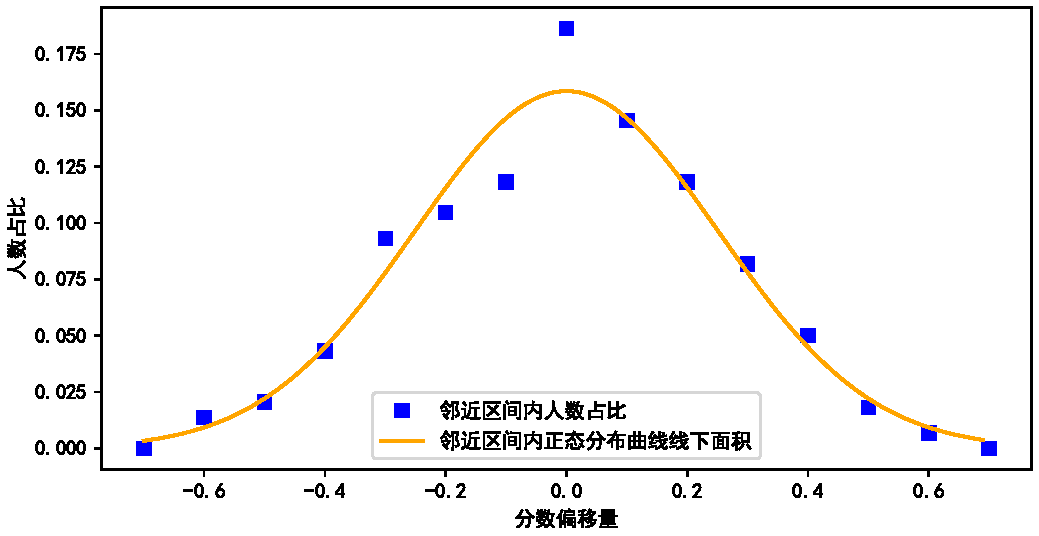
\includegraphics[width=\textwidth]{fig/fittingOffsets.pdf}
            \caption{散点图和拟合结果}
            \label{fig:fittingOffsetsByNormalDistribution}
        \end{figure}

        \vspace{1.5ex}

        图\ref{fig:fittingOffsetsByNormalDistribution}展示了拟合的结果。可以看到,除了约$3$个数据点以外,其余数据点均与曲线贴合紧密。为了验证这些数据是否确实服从正态分布,还需绘制Q-Q图来进行检验。

        \begin{figure}
            \centering
            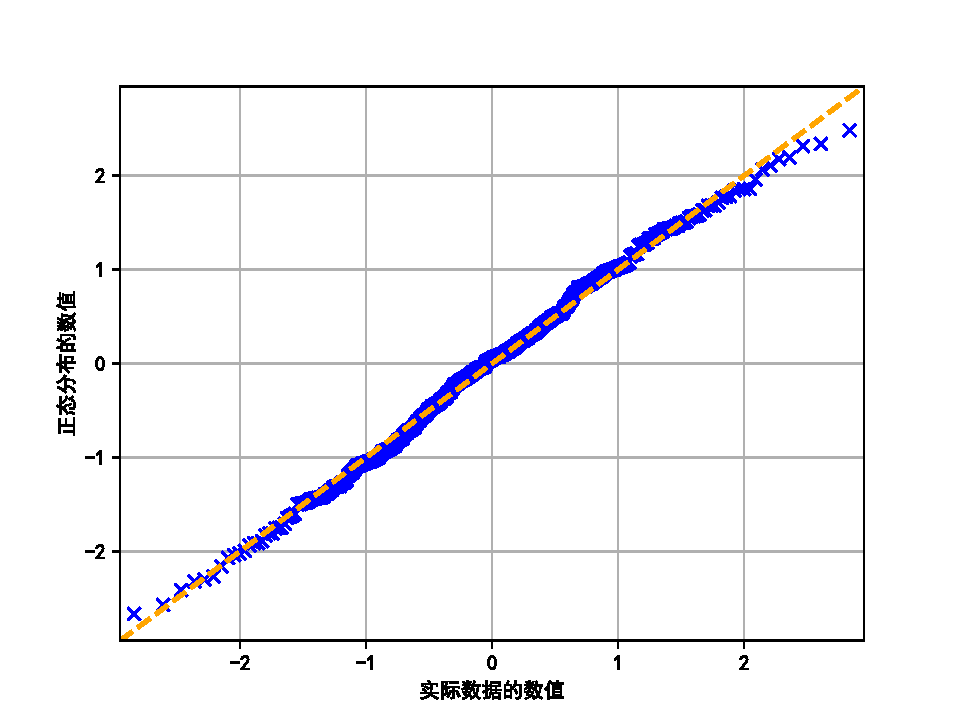
\includegraphics[width=\textwidth]{fig/QQPlot.pdf}
            \caption{Q-Q图,关于比赛分数差值数据和正态分布绘制}
            \label{fig:QQPlot}
        \end{figure}

        \vspace{1.5ex}

        图\ref{fig:QQPlot}展示了所绘制的Q-Q图。注意,该图的坐标轴经过缩放,故坐标轴上标注的数值仅能代表相对的比例关系。
        
        图\ref{fig:QQPlot}中有440个蓝色叉号,所有叉号的横坐标、纵坐标非严格递增。其中第 $k$ 个叉号($1\leq k\leq 440$)对应着440个数值中的第 $k$ 小值 $\textit{val}_k$ ,叉号的横坐标 $x_k$ 等于对应的数值 $\textit{val}_k$ ,而叉号的纵坐标 $y_k$ 等于:440个服从正态分布 $N(0,\sigma^2)$ 的数值中,第 $k$ 小值的期望;其中的 $\sigma$ 是待定的参数。可以证明 $y_k$ 满足 $R_{\sigma^2}(y_k)=\frac {k}{440+1}$ ,于是由这一关系可以求出 $y_k$ 。

        如果这440个数值服从 $N(0,\sigma^2)$ 的话,容易想到应该有 $x_k\approx y_k$ ,也就是说所有叉号落在直线 $y=x$ 附近。我们通过选取合适的 $\sigma>0$ 来让叉号尽可能贴近直线 $y=x$ ,最终的结果就是图\ref{fig:QQPlot}。可以看到,叉号与直线紧密贴合,所以这些数据确实服从正态分布\footnote{注意到,缩放坐标轴和改变 $\sigma$ 的取值,这两种操作对图像的改变其实是完全相同的,所以缩放坐标轴不会影响结论的可靠性}。又由假设\ref{ass:similarityOfDeltaDistributions},这一规律对任何COI/IOI赛制的比赛都成立。

        \begin{theorem}[偏移量分布的形式]
            对任何基于COI或IOI赛制的现实比赛,其对应的理想比赛的偏移量分布是期望值为$0$的正态分布。
            \label{thm:normalityOfOffsetsDistribution}
        \end{theorem}

\section{选手整体水平的估计}

    本节将借助联赛初赛(字母标号a)和联赛复赛(字母标号b)的分数数据,来估计全国信息学竞赛选手整体水平的分布情况。

    \subsection{对复赛分数的分析}

        选手的“水平”是一个模糊的概念;为了将其量化,我们将用一名选手在联赛复赛中的期望分数来衡量这名选手的水平。

        虽然由假设\ref{ass:equivalenceBetweenCodingContests},不同年份的联赛复赛(所对应的理想比赛)是缩放等价的;但它们毕竟不相同,因此“在联赛复赛中的期望分数”这一概念需要澄清。\ref{sec:dataPreprocessingOfNOIP}小节将处理这一问题,并完成对复赛分数数据的初步分析。接着,\ref{sec:calculatingXfromC}小节将从这些数据中得到联赛复赛(所对应的理想比赛)的期望值分布的表达式。

        由此得到的期望值分布仍不是真实的结果,因为联赛初赛在此之前已经筛选掉了一部分选手。对这一影响的处理是\ref{sec:analysisOnPreliminaryRound}小节的任务。

        \subsubsection{数据的获取、加工和拟合}\label{sec:dataPreprocessingOfNOIP}

            数据来自以下6场比赛:
            \begin{asparaitem}
                \item NOIP2016\ ---\ 复赛(字母标号b)
                \item NOIP2017\ ---\ 复赛(字母标号b)
                \item NOIP2018\ ---\ 复赛(字母标号b)
                \item CSP2019\ ---\ 复赛(字母标号b)
                \item CSP2020\ ---\ 复赛(字母标号b)
                \item NOIP2020\ ---\ 复赛(字母标号b)\footnote{2020年情况较为特殊,NOIP与CSP同时存在,且NOIP初赛与CSP初赛合并为同一场比赛}
            \end{asparaitem}

            \vspace{1.5ex}

            之所以只采用2016年及以后的比赛,是出于两个原因:
            \begin{asparaitem}
                \item 年代过于久远的比赛对当今的参考意义有限。
                \item 仅有的数据来源为NOI官网上的获奖名单公示,故只能取得\emph{获奖选手}的分数信息。而自2016年起CCF更改了获奖规则,增加了获奖人数,使得可以获取的数据量大了许多。
            \end{asparaitem}

            \vspace{1.5ex}

            \begin{table}\footnotesize
                \centering
                \begin{tabular}{@{}lccccc@{}}
                    \toprule
                     & \multicolumn{1}{l}{参赛人数} & \multicolumn{1}{l}{获奖人数} & \multicolumn{1}{l}{满分} & \multicolumn{1}{l}{最高分} & \multicolumn{1}{l}{获奖分数线} \\ \midrule
                    NOIP2016复赛 & 约8300  & 约5900 & 600 & 600 & 100 \\
                    NOIP2017复赛 & 约10300 & 约6600 & 600 & 600 & 80  \\
                    NOIP2018复赛 & 约12900 & 约8000 & 600 & 600 & 120 \\
                    CSP2019复赛  & 约13900 & 约8800 & 600 & 600 & 80  \\
                    CSP2020复赛  & 约11000 & 约6700 & 400 & 400 & 30  \\
                    NOIP2020复赛 & 约4700  & 约3600 & 400 & 400 & 60  \\ \bottomrule
                \end{tabular}
                \caption{6场比赛的相关数据}
                \label{tab:noip16to20}
            \end{table}

            表\ref{tab:noip16to20}展示了关于这6场比赛的几项统计数据。

            \vspace{1.5ex}

            由假设\ref{ass:equivalenceBetweenCodingContests},这6场现实比赛(所对应的理想比赛)是缩放等价的。进而由命题\ref{prop:alphaAsQuotientOfStddev},这6场现实比赛所对应的理想比赛,在对分数作变换(变换方式见\ref{sec:dataPreprocessingOfCTT}小节)后,将成为完全相同的理想比赛。

            于是,与\ref{sec:dataPreprocessingOfCTT}小节类似,数据加工将按以下步骤进行:
            \begin{asparaenum}[\bfseries{步骤} 1.]
                \item 将所有比赛中所有选手的分数除以当场比赛的最高分(也就是计算标准分;注意到最高分等于满分),用以代替原始分数。
                \item \label{step:noipDataRefinementStep2} 去除所有$<0.2$的分数。这是因为在这6场比赛中,获奖分数线与最高分的商的最大值为$0.2$;这意味着分数低于$0.2$的选手中有一部分未能获奖,于是这些选手中其余部分的数据也失去意义,因此一并剔除。
                \item 对每场比赛计算分数标准差 $\sigma$ ,然后对分数作变换 $x\mapsto 1-\frac{1-x}{5.52\sigma}$ ,并用变换结果代替原分数。使用系数$5.52$的理由稍后说明。
                \item 对每场比赛计算最低分,取所得的6个最低分的最大值$T$,并剔除所有$<T$的分数。这一步的理由与步骤\ref{step:noipDataRefinementStep2}中的类似:分数低于$T$的部分选手未能获奖,故将这些选手连同已获奖的那些一并剔除。计算可得 $T\approx 0.200$ ,与步骤\ref{step:noipDataRefinementStep2}中的阈值保持一致;这正是系数$5.52$的主要作用。
                \item 现在所有这些分数数据属于同一理想比赛 $A$ (满足 $A$ 与原先6个现实比赛所对应的理想比赛缩放等价),将它们汇集起来即可。注意到我们所取得的并非完整的分数数据,而只是$\geq 0.2$的那一部分分数。
            \end{asparaenum}

            \vspace{1.5ex}

            本节中我们约定使用理想比赛 $A$ 作为衡量选手水平的标尺,即我们将用一名选手在 $A$ 中的期望分数,来代表该名选手的水平。

            \vspace{1.5ex}

            经过上述加工后,我们得到了26907个落在$[0.2,1]$之中的分数数据。由命题\ref{prop:scoreDistributionMeaning},这些数据应当服从 $\bm{C}_A$ 所描述的概率分布。
            
            受数据限制,我们暂时只关心 $[0.2,1]$ 这一分数区间上的分布情况。即我们要确定函数 $F:\left[0.2,1\right]\to\mathbb{R}_{\geq 0}$ ,满足在任何一个区间 $\left[a,b\right]$ 上,$F$ 的定积分在数值上约等于:落在$\left[a,b\right]$中的分数数值个数,与数值总个数26907的比值。注意到在$F$和$\bm{C}_A$之间有这一关系:$$F(t)=\bm{C}_A(t)\Big/{\displaystyle\int\limits_{0.2}^1 \bm{C}_A(x)\mathrm{d}x},\quad\forall t\in[0.2,1]$$

            观察这些数据,可以发现数值的分布左侧(即靠近$0.2$一侧)稠密、右侧(即靠近$1$一侧)稀疏,于是尝试用递降的多项式函数、对数函数等常见函数,以及指数分布、截尾正态分布等“向左倾斜”的常见概率分布来拟合之。实验发现使用对数函数的拟合效果大幅好于其他方式,以下将描述对数函数的拟合过程和结果。

            \begin{enumerate}[leftmargin=6em]
                \item [\textbf{步骤 1.}] 对于 $t=0.25,0.30,\cdots,0.95$ ,计算:落在 $\left[t-0.05,t+0.05\right]$ 中的数值个数与总个数26907的比值。这个比值记为 $c(t)$ 。
                \item [\textbf{步骤 2.}] 在平面直角坐标系中画出 $t-c(t)$ 散点图。
                \item [\textbf{步骤 3.}] 选取参数 $\alpha$ 并令 $F(x)=\alpha\log(x)$ 。注意到函数 $F$ 在 $[0.2,1]$ 上的定积分必须等于$1$,由此可唯一确定 $\alpha$ 的取值;计算得到 $\alpha\approx-2.09156$ 。
                \item [\textbf{步骤 4.}] 检查函数 $$G(t)=\int\limits_{t-0.05}^{t+0.05}F(x)\mathrm{d}x$$ 的图像是否与 $t-c(t)$ 散点图吻合。
            \end{enumerate}

            \begin{figure}
                \centering
                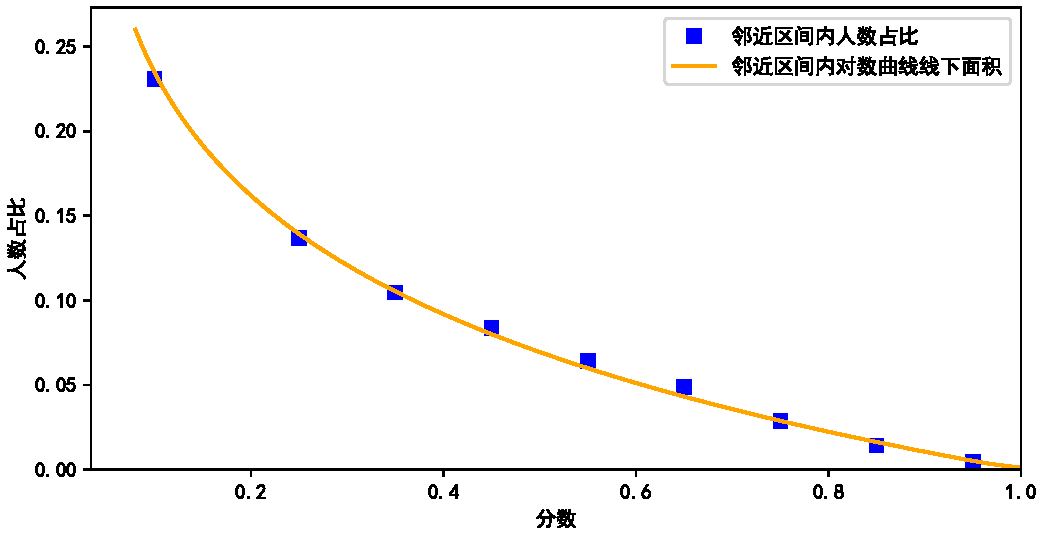
\includegraphics[width=\textwidth]{fig/fittingNoipScores.pdf}
                \caption{散点图和拟合结果}
                \label{fig:fittingNoipScoresByLogCurve}
            \end{figure}

            图\ref{fig:fittingNoipScoresByLogCurve}展示了拟合的结果。可以看到全部数据点与曲线贴合紧密,且算得残差平方和约为$3.3\cdot 10^{-4}$,显示出了较好的拟合效果。基于此,我们确定取 $F(x)=\alpha\log(x)$ ,其中 $\alpha\approx-2.09156$ 。

            我们推测在区间 $\left[0,0.2\right)$ 上,分数的分布依旧近似地符合对数曲线的形态。假定如此,则分数区间 $[0.2,1]$ 上的人数占总人数的比例应该等于 $$\dfrac{\displaystyle\int\limits_{0.2}^1 \log(x)\mathrm{d}x}{\displaystyle\int\limits_0^1 \log(x)\mathrm{d}x}\approx 0.478$$ 进而根据分数区间 $[0.2,1]$ 上的总人数为26907,可推算出(前述6场比赛的)参赛总人数约为56300。该值与真实值61100接近,于是我们的假设得到验证。

            由此可知 $A$ 的分数分布函数的表达式同样形如 $\bm{C}_A(x)=\beta\log(x)$ ,其中系数 $\beta$ 可由等式 $$\int\limits_0^1 \bm{C}_A(x)\mathrm{d}x=1$$ 唯一确定;计算得 $\beta=-1$ 。

            \begin{proposition}
                $\bm{C}_A(x)=-\log(x)$ ,其中 $A$ 是根据\ref{sec:dataPreprocessingOfNOIP}小节中描述的过程所确定的理想比赛。
                \label{prop:scoreDistributionOfStandardizedNoip}
            \end{proposition}
            
        \subsubsection{从分数分布计算期望值分布}\label{sec:calculatingXfromC}

    \subsection{结合初赛分数的分析}\label{sec:analysisOnPreliminaryRound}